\subsection{Complétion cubique typée de l’espace ambiant régional}
\label{vi:cubo:completacion}

La complétion admet une description ensembliste qui explicite son
opération. Soit \(E_9\) l'ensemble des neuf classes résiduelles, représentées
positivement par \(1,\ldots,9\), et soit \(\ast\) un élément supplémentaire.
Le symbole \(\ast\) est distinct de la classe nulle, déjà représentée par \(9\).
Par conséquent, l'extension de \(E_9\) à
\(\widehat E=E_9\sqcup\{\ast\}\) porte le cardinal de neuf à dix
sans modifier l'identification modulaire interne. La complétion cubique est
\(\widehat C=\widehat E^3\), et le cube initial est \(C=E_9^3\).

L’espace ambiant régional déjà construit par \(\Psi\) dans
\eqref{eq:psi-catalogo}, dont le recensement exact est établi par la
Proposition~\ref{vi:reg:censo}, est \(\FF_3^6\). Pour typer sa résidence
dans le cube initial, nous écrivons \([a]_3\in\{0,1,2\}\)
pour le représentant de \(a\in\FF_3\) et fixons la bijection
\[
 \eta:\FF_3^2\longrightarrow E_9,
 \qquad \eta(a,b)=1+3[a]_3+[b]_3.
\]
Le regroupement par paires
\begin{equation}
 \beta(w_1,\ldots,w_6)=
 \bigl(\eta(w_1,w_2),\eta(w_3,w_4),\eta(w_5,w_6)\bigr)
 \label{vi:cubo:beta}
\end{equation}
est donc une bijection \(\FF_3^6\to E_9^3=S_0\). En particulier,
les \(243\) mots produits par le recensement précédent résident dans le corps
initial de \(729\) positions ; ni \(\eta\) ni \(\beta\) ne sélectionnent une
région, une espèce physique ou une valeur métrologique. La sélection régionale
est une étape postérieure et distincte, démontrée dans la
Proposition~\ref{vi:reg:seleccion}. L’égalité numérique
\(|\operatorname{im}\Psi|=|S_1|=243\) n’identifie pas les deux ensembles :
\(\beta(\operatorname{im}\Psi)\) est un sous-ensemble de \(S_0\), tandis
que \(S_1\) appartient à la couronne d’agrandissement.

\subsubsection{Différence de seuil et composition des couronnes}
\label{vi:cubo:mg07:umbral}

L'extension d'une cellule discrète conserve toutes les strates qui
apparaissent lorsqu'on augmente sa taille d'une unité. La différence de seuil
exprime cette opération sur le lecteur de cardinaux et permet de suivre
son comportement sous l'addition et la multiplication avant d'introduire une
réalisation métrique.

\begin{definition}[Différence de seuil]
Soit \(R\) un anneau commutatif unitaire et soit
\(f:\mathbb Z_{\geq0}\to R\). Nous définissons
\begin{equation}
 (D_\#f)(n)=f(n+1)-f(n).
 \label{vi:cubo:mg07:definicion}
\end{equation}
Pour un lecteur entier de cellules finies emboîtées, cette différence
enregistre le cardinal de la couronne incorporée à l'étape \(n\to n+1\).
\end{definition}

\begin{proposition}[Additivité et loi exacte du produit]
Pour \(f,g:\mathbb Z_{\geq0}\to R\), on a
\begin{align}
 D_\#(f+g)(n)&=D_\#f(n)+D_\#g(n),
 \label{vi:cubo:mg07:aditividad}\\
 D_\#(fg)(n)&=f(n+1)D_\#g(n)+g(n)D_\#f(n)
 \label{vi:cubo:mg07:producto-desplazado}\\
 &=f(n)D_\#g(n)+g(n)D_\#f(n)
   +D_\#f(n)D_\#g(n).
 \label{vi:cubo:mg07:producto}
\end{align}
\end{proposition}

\begin{proof}
La différence de la somme se sépare terme par terme. Pour le produit,
ajouter et soustraire \(f(n+1)g(n)\) donne
\[
 \begin{split}
 f(n+1)g(n+1)-f(n)g(n)
 &=f(n+1)\bigl(g(n+1)-g(n)\bigr)\\
 &\quad+g(n)\bigl(f(n+1)-f(n)\bigr).
 \end{split}
\]
Cela prouve \eqref{vi:cubo:mg07:producto-desplazado}. La substitution
\(f(n+1)=f(n)+D_\#f(n)\) produit
\eqref{vi:cubo:mg07:producto} avec son terme bilinéaire complet.
\end{proof}

Si \(A_n\subseteq A_{n+1}\) et \(B_n\subseteq B_{n+1}\) sont des
ensembles finis, la couronne du produit se décompose en trois parties
disjointes :
\[
 \begin{split}
 (A_{n+1}\times B_{n+1})\setminus(A_n\times B_n)
 &=\bigl(A_n\times(B_{n+1}\setminus B_n)\bigr)\\
 &\quad\sqcup\bigl((A_{n+1}\setminus A_n)\times B_n\bigr)\\
 &\quad\sqcup\bigl((A_{n+1}\setminus A_n)
                 \times(B_{n+1}\setminus B_n)\bigr).
 \end{split}
\]
Prendre les cardinaux donne exactement \eqref{vi:cubo:mg07:producto}. Le terme
bilinéaire compte les positions nouvelles dans les deux facteurs ; son lieu de résidence
est l'intersection des deux extensions, avec l'incidence conservée.

\begin{proposition}[Loi binomiale de la couronne dimensionnelle]
Pour \(d\geq1\), soit \(f_d(n)=n^d\). Alors
\begin{equation}
 D_\#f_d(n)=(n+1)^d-n^d
 =\sum_{k=0}^{d-1}\binom dk n^k
 =\sum_{r=1}^{d}\binom dr n^{d-r}.
 \label{vi:cubo:mg07:binomio}
\end{equation}
\end{proposition}

\begin{proof}
Le développement binomial de \((n+1)^d\) contient \(n^d\) et les \(d\) termes restants de la première somme. La substitution \(r=d-k\) donne la seconde. Sur le support \(\{1,\ldots,n+1\}^d\), chaque position ajoutée possède un ensemble non vide de coordonnées égales à \(n+1\). Si cet ensemble contient \(r\) éléments, il y a \(\binom dr\) choix de positions et \(n^{d-r}\) choix des coordonnées précédentes. Ces strates sont disjointes et couvrent la couronne ; elles prouvent donc également la formule par incidence finie.
\end{proof}

Pour \(d=3\), les trois strates ont les cardinaux \(3n^2\),
\(3n\) et \(1\). Au passage nonadique--décimal, \(n=9\), l'
opération donne \(243+27+1=271\) ; l'exclusion du sommet final laisse
\(270\) positions. La complétion cubique qui suit explicite l'
union de cette couronne avec les \(729\) positions antérieures. La loi
de seuil conserve ainsi tant le total que la répartition selon le nombre
de nouvelles coordonnées. Les réalisations réticulaires ultérieures
transportent leurs incidences au moyen des applications spécifiques de chaque
construction.


\begin{definition}[Strates de codimension combinatoire]
Pour \(0\leq r\leq3\), on définit
\[
 S_r=\{(x_1,x_2,x_3)\in\widehat E^3:
             \#\{j:x_j=\ast\}=r\}.
\]
L'apex de la complétion est \(a_\ast=(\ast,\ast,\ast)\), et la
complétion poncturée est \(\widehat C^{\circ}=\widehat C\setminus\{a_\ast\}\).
\end{definition}

\begin{proposition}[Décomposition exacte de la complétion]
Les strates sont disjointes et satisfont
\begin{align}
 \widehat C&=S_0\sqcup S_1\sqcup S_2\sqcup S_3,
 &|S_r|&=\binom3r9^{3-r},\label{vi:cubo:estratos}\\
 |\widehat C^{\circ}|&=729+243+27=999,
 &|\widehat C|&=999+1=729+271=1000.\label{vi:cubo:999}
\end{align}
L'extension poncturée contient \(270\) éléments supplémentaires par rapport au cube
initial ; l'extension complète en contient \(271\).
\end{proposition}
\begin{proof}
Un élément de \(S_r\) s'obtient en choisissant les \(r\) coordonnées qui
contiennent \(\ast\), de \(\binom3r\) façons, puis en attribuant aux autres
l'une des neuf classes de \(E_9\). La classification selon le nombre de
coordonnées supplémentaires est exhaustive et ses classes sont disjointes. L'unique
élément de \(S_3\) est \(a_\ast\). Le retirer soustrait une unité au cardinal
total ; le restituer rétablit le produit cartésien complet.
\end{proof}

L'expression \emph{extrême et moyenne raison holographique}, abrégée EMRH dans
le corpus, désigne ici cette articulation entre le corps initial, les
strates d'extension et la restitution unitaire. Son contenu immédiat
est la partition exacte d'un produit fini et sa normalisation. Le nombre
\(999\) représente un objet déterminé, la complétion poncturée ;
\(1000\) représente sa clôture par restitution de l'apex. L'unité
ajoutée possède donc une résidence d'incidence explicite.

\begin{figure}[htbp]
\centering
\begin{tikzpicture}[x=1cm,y=1cm,>=Stealth,font=\small]
\draw[->] (0,0)--(12.4,0);
\foreach \x/\a/\b in {0/729/{S_0},4.0/243/{S_1},7.5/27/{S_2},10.6/1/{S_3}}{
  \draw (\x,0.12)--(\x,-0.12);
  \node[above=5pt] at (\x,0) {\(\a\)};
  \node[below=5pt] at (\x,0) {\(\b\)};
}
\draw[decorate,decoration={brace,amplitude=5pt}] (0,1)--(7.7,1);
\node[above=8pt] at (3.85,1) {Complétion poncturée : \(999\)};
\draw[decorate,decoration={brace,mirror,amplitude=5pt}] (0,-1)--(10.8,-1);
\node[below=8pt] at (5.4,-1) {Complétion intégrale : \(1000=999+1\)};
\node[align=center] at (10.6,1.5) {Apex\\\((\ast,\ast,\ast)\)};
\end{tikzpicture}
\caption{Strates de la complétion cubique. La disposition représente
la décomposition ensembliste, non une échelle métrique. Les \(243\) éléments
de \(S_1\) forment trois strates coordonnées de \(81\) éléments ; les \(27\)
de \(S_2\), trois strates de \(9\). L'apex complète la partition.}
\label{vi:cubo:estratos-fig}
\end{figure}

% Inclusión de la figura histórica vectorial en escala de grises.
% El PDF y su fuente standalone se conservan literalmente como cubo_emrh_original.*.
\begin{figure}[htbp]
\centering
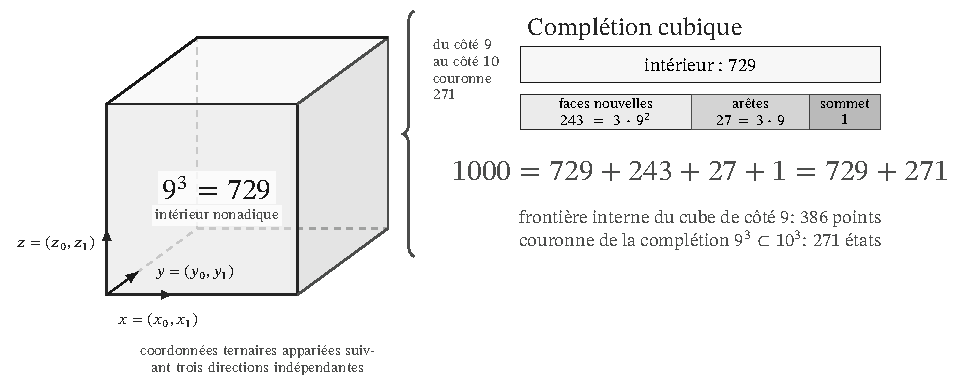
\includegraphics[width=\textwidth]{figures/cubo_emrh_original.pdf}
\caption{Représentation cubique de l'extension de neuf à dix classes par coordonnée. Les strates \(S_1,S_2,S_3\) placent les incidences ajoutées sur les faces, les arêtes et l'apex ; leurs cardinaux forment la couronne de \(271\) éléments. La frontière de \(386\) éléments appartient au cube initial. La perspective géométrique complète la partition de la figure ~\ref{vi:cubo:estratos-fig} ; les séparations graphiques ont une fonction schématique.}
\label{vi:cubo:completacion-3d}
\end{figure}


\subsubsection{Conservation de l'unité et compatibilité dimensionnelle}

La normalisation ne se limite pas à diviser une identité isolée. En dimension
\(d\), le produit \(\widehat E^d\) porte la mesure uniforme
\(\mu_d(\{x\})=10^{-d}\). La projection coordonnée
\(p_d:\widehat E^{d+1}\to\widehat E^d\) supprime la dernière coordonnée.

\begin{proposition}[Compatibilité projective des mesures normalisées]
Pour tout \(d\geq1\),
\[
 (p_d)_*\mu_{d+1}=\mu_d,
 \qquad \mu_d(\widehat E^d)=1.
\]
La masse de la strate comportant \(r\) coordonnées supplémentaires est
\(\binom dr9^{d-r}/10^d\), et la somme des masses de toutes les strates
vaut un.
\end{proposition}
\begin{proof}
Chaque point de \(\widehat E^d\) possède dix préimages. Leur masse totale est
\(10\,10^{-(d+1)}=10^{-d}\). L'égalité pour tout sous-ensemble
s'obtient en sommant sur ses points. La formule stratifiée provient
du même dénombrement que \eqref{vi:cubo:estratos} ; le binôme
\((9+1)^d\) donne la normalisation totale.
\end{proof}

En dimension trois, retirer l'apex laisse une masse \(999/1000\), et
le restituer ajoute \(1/1000\). Renormaliser avant la restitution
définirait une autre mesure : la distinction est pertinente sur le plan opératoire.
En particulier, conservation de la masse probabiliste, conservation des
registres de transport et dissipation thermodynamique sont des affirmations portant sur
des objets différents. La proposition démontre la première et fournit le
support compatible pour étudier la deuxième ; la troisième requiert une
réalisation dynamique et énergétique spécifiée.

La frontière géométrique interne demeure également distincte.
Sur le représentant cartésien \(\{1,\ldots,9\}^3\), retirer
\(\{2,\ldots,8\}^3\) laisse \(386\) points. Cette frontière appartient au
cube initial, tandis que \(\widehat C\setminus C\) appartient à son
extension. La complétion cubique, le développement positionnel en base mille et
la lecture d'incidence exceptionnelle partagent des données du support ;
leurs applications respectives déterminent l'information issue de ces données qu'utilise
chaque représentation.
